\documentclass[a4paper,12pt,final]{article}


\usepackage{graphicx}
\title{
\begin{center}
  	
\includegraphics[scale=0.3]{Logo.png} 
  \end{center}
  \textbf{\\}
Iteration 1\\
}
\author{101 Solutions}

\begin{document}

\maketitle
\thispagestyle{empty}
\newpage
\tableofcontents
\thispagestyle{empty}
\newpage
\pagenumbering{arabic}

\section{Introduction}
The purpose of this document is to keep track of the ongoing development progress of the software application manager AppMan.  In each iteration additional content will be added which will result in this document being an up to date and relaible method to view progress and current development plans and ideas. Content will include milestones reached, current goals and the current functionality of the software.

\section{Milestones reached}
\begin{itemize}
\item Successfully tendered and accepted to complete this project
\item Completed vision and scope document
\item Completed an arcitechtural design and documentation
\item Completed a prototype GUI for AppMan
\item Partially implemented a backend system
\end{itemize}


\section{Immediate Goals}
Our next two main goals for the project:
\subsection{Server \& Client network communication}
\begin{itemize}
\item Goal: To create a reliable socket connection between the server and client applications, which will serve as a pathway between them.
\end{itemize}
\subsection{Build transference}
\begin{itemize}
\item Goal: To establish a list of builds which will be recognized by the server application and the ability to copy the builds to the clients(Slave computers)
\end{itemize}
\subsection{Build Information Storage}
\begin{itemize}
\item Goal: Creating a database that can store information related to builds kept on the master and slaves
\end{itemize}
\subsection{Slave Application}
\begin{itemize}
\item Goal: Creating a program that will communicate with the Master application
\end{itemize}


\section{Functionality}
\subsection{Graphic User Interface}
\begin{itemize}
\item A gui built in c++ and QT and deployable in both windows and linux.
\item Easy to understand gui layout used
\item A help form that will describe some of the workings of the program. This form will display how to add a build, and understand how the program works, etc
\item Drag and drop capability on the gui, which will be incorporated with further development
\begin{itemize}
\item Dragging the "drag" label to copy a build from master to slave(future development)
\item Dropping a file or directory on the "+ Add" Button(future development)
\end{itemize}
\item Gui is capable running with or without the images that are to be deployed with it
\item Gui Caters for other development
\begin{itemize}
\item Copy files over from master to slave( with a progressbar indicating the file copy progress )
\item Running applications that have been copied to slave computers
\item SpinBoxes that can allow a large amount of slave computers or builds to be shown by the program
\end{itemize}
\end{itemize}

\section{System Design}
\subsection{AppMan}

\begin{center}
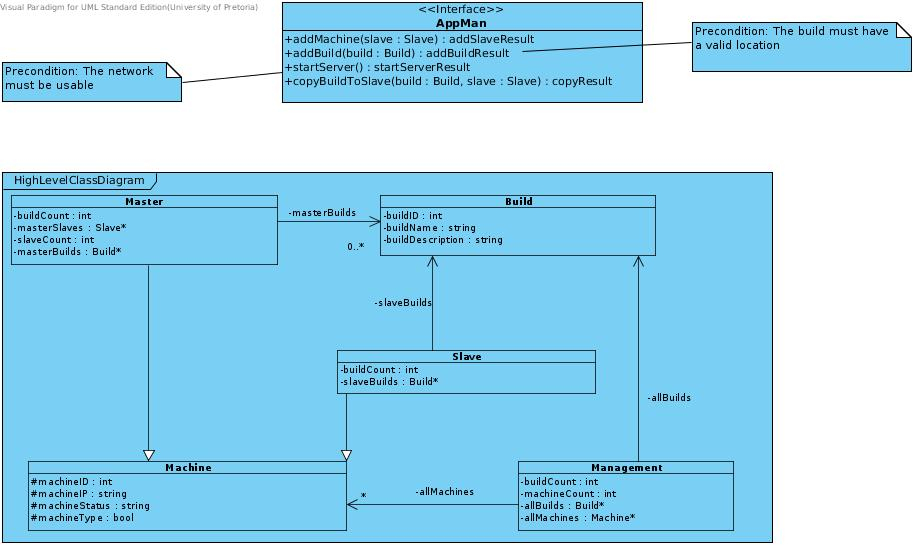
\includegraphics[scale=0.5]{AppManDiagram.jpg} 
\end{center}

\subsection{AppManClient}

\begin{center}
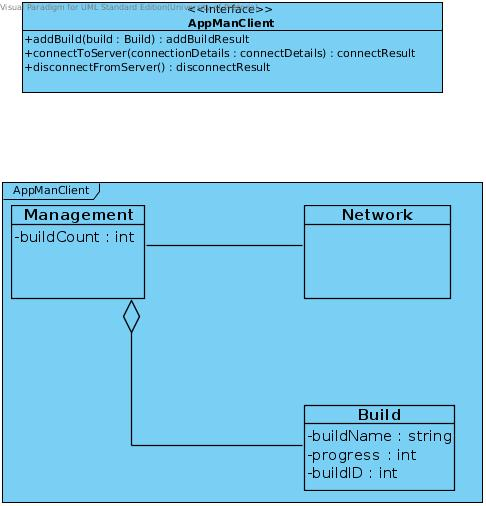
\includegraphics[scale=0.5]{AppManClientDiagram.jpg} 
\end{center}

\section{Processes}
\subsection{ActivityDiagram}
%%%%activity diagram possibly hier

\section{Functional Requirements}
\subsection{Use Case Diagrams}
\begin{itemize}
\item AppMan\\
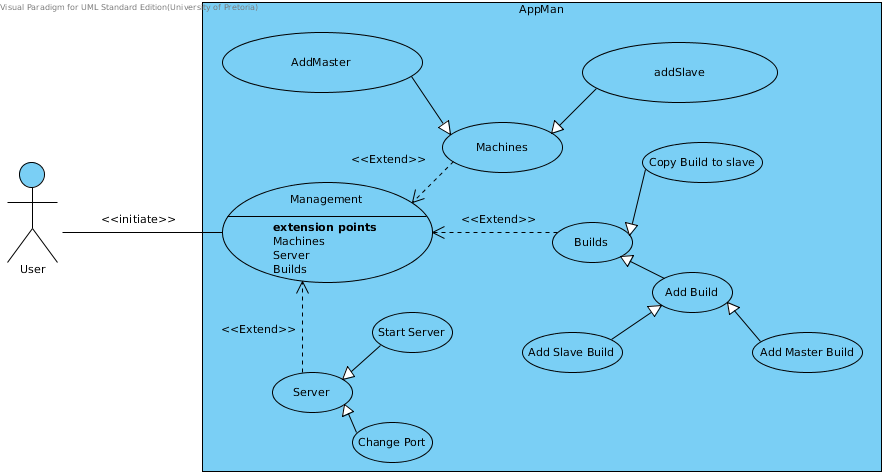
\includegraphics[scale=0.5]{UseCaseDiagram.png} 
\item AppManClient\\
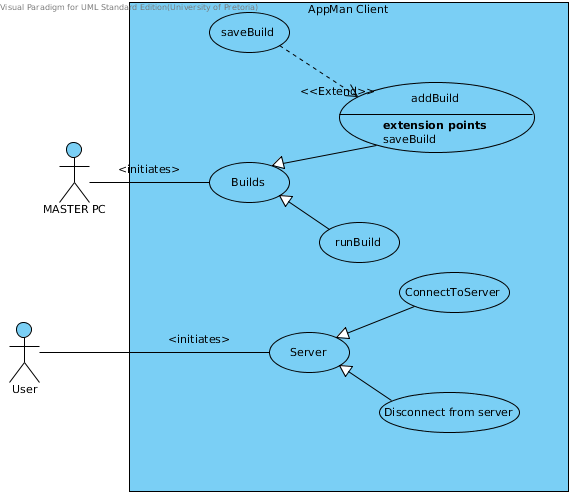
\includegraphics[scale=0.6]{UseCaseDiagramClient.png} 
\end{itemize}

\subsection{Builds}
\begin{itemize}
\item Builds must be addable to the master
\item Builds must be updated on the slave computers once a change have been made
\item Only changed files must be sent to the slave computers once a change has been made
\item Easy to manage the builds that are on the master computer
\item Builds must be able to have the following
\begin{itemize}
\item Name
\item Directory
\end{itemize}
\end{itemize}

\subsection{Copying}
\begin{itemize}
\item Copying must be done over the network
\item The copy of multiple files must be compressed to reduce the time it takes to copy a file
\item Progress of copy must be shown on master computer while copying takes place
\end{itemize}

\subsection{User Interface}
\begin{itemize}
\item The user interface must be easy to use
\item The user interface must make use of drag and drop capabilities to promote usability
\end{itemize}

\subsection{Slave Computers}
\begin{itemize}
\item Slave computers must connect to the master computer via the network
\end{itemize}

%Header dan class diagram
%Dink die package diagram vervang die class diagram


\section{Glossary}
\begin{itemize}
\item Build - An application build version that could potentially be distributed to slave computers
\item Slave - A computer that will be controlled via a master computer
\item Application builds will be sent to this computer
\item Master - A computer that will control Slaves across a network
\item Server - A machine waiting on the network for connections from other machines
\item GUI - Graphical User Interface with which a user can control the project
\item Project - This project. The distributed application manager
\item Application Configuration - Environment variables that are specified when running an application
\end{itemize}


\end{document}